\section{Auswertung}

In dem folgenden Abschnitt sollen mithilfe der aufgenommenen Daten die Lebensdauer
der Myonen bestimmt werden. Die Fehlerberechnung wird im folgenden mit dem
Package $\textit{uncertainties}$ in $\textit{Python}$ durchgeführt. Da die Werte
bei Berechnung des Plateaus sowie Ermittlung der Lebensdauer Fehlerbehaftet sind,
wird für die Regression ein gewichteter Fit mit der Funktion \textit{curve\_fit}
durchgeführt.

\subsection{Einstellung der Verzögerungszeit}

Um die abgegebenen Signale der Koinzidenzapparatur zu maximieren, wird während
der Kalibrierung des Versuches die Verzögerungszeit $T\ua{VZ}$ varriert. Die am
Ausgang der Apparatur gemessene Anzahl an Signalen wird in Tabelle \ref{tab:Verzögerung}
wiedergegeben und ist in Abbildung \ref{fig:Plateau}graphisch dargestellt.
In den interessanteren Bereichen wurden mehrere Messwerte genommen, allerdings
ist in Tabelle \ref{tab:Verzögerung} immer nur der gemittelte
Wert eingetragen. Die jeweiligen Zeiten sind mit einem Sternchen markiert. Ein
negatives Vorzeichen bei der Verzögerungszeit entspricht einer Verzögerung bei
dem linken SEV und ein positives Vorzeichen dementsprechend einer Verzägerun
bei dem rechten SEV. Da es sich um eine Anzahl handelt, sind die Zahlen auf
die 1er Potenz gerundet. Als Fehler wird für den Wert $n$ immer $\sqrt{n}$
angenommen.

\begin{figure}
  \centering
  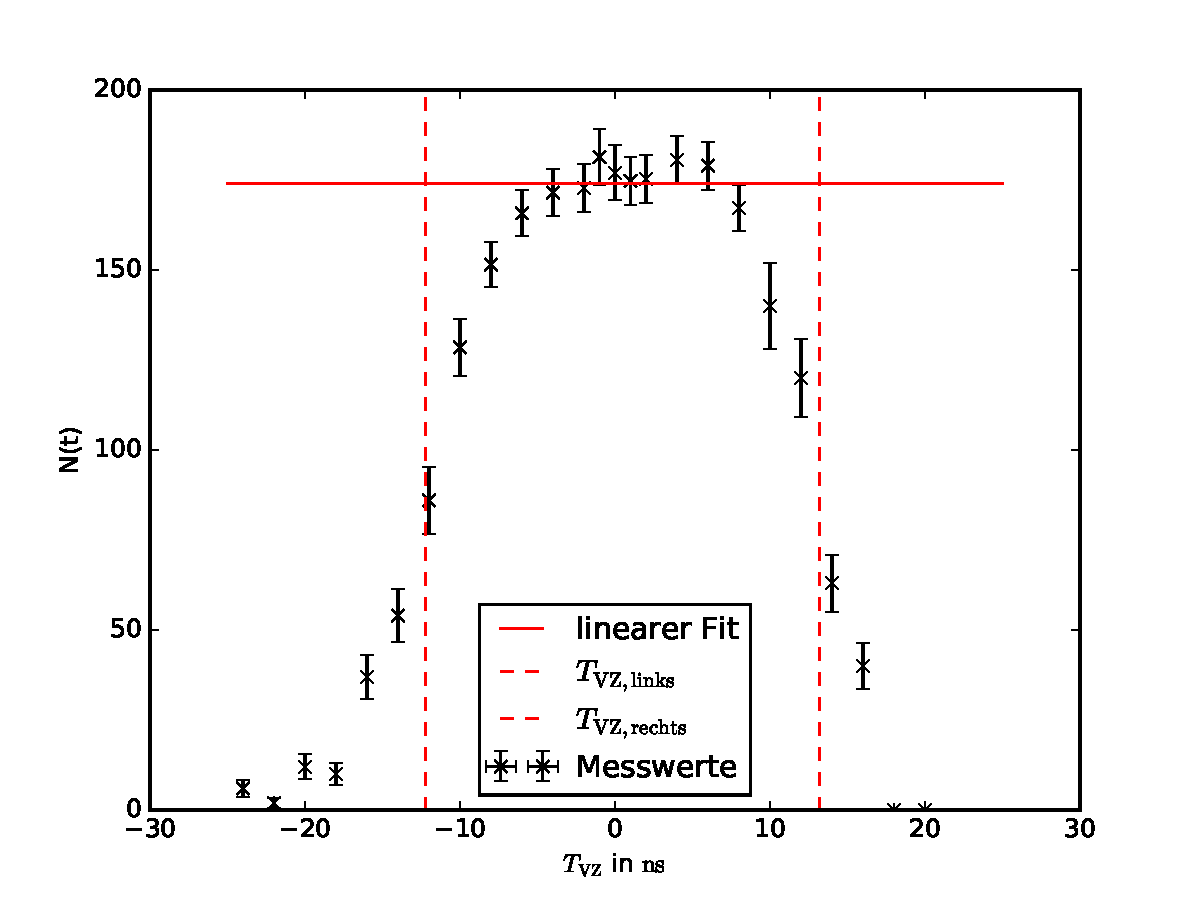
\includegraphics[width = \textwidth]{Pics/Plateau.pdf}
  \caption{Plateau für die Impulsrate bei varrierter Verzögerungszeit.}
  \label{fig:Plateau}
\end{figure}

\begin{table}
  \centering
  \caption{Messwerte bei Einstellung der Verzögerungszeit.}
  \label{tab:Verzögerung}
  \begin{tabular}{c c c c}
    \toprule
    $T\ua{VZ}$ in $\su{ns}$ & $N(T\ua{VZ})$ $\pm$ $\increment N$ &
    $T\ua{VZ}$ in $\su{ns}$ & $N(T\ua{VZ})$ $\pm$ $\increment N$  \\
    \midrule
    -24  &  6  $\pm$ 2  & 0*   & 177 $\pm$ 8  \\
    -22  &  2  $\pm$ 1  & 1*   & 175 $\pm$ 7  \\
    -20  & 12  $\pm$ 3  & 2*   & 176 $\pm$ 7  \\
    -18  & 10  $\pm$ 3  & 4*   & 181 $\pm$ 7  \\
    -16  & 37  $\pm$ 6  &  6*  & 179 $\pm$ 7  \\
    -14  & 54  $\pm$ 7  & 8*   & 168 $\pm$ 6  \\
    -12  & 86  $\pm$ 9  & 10   & 140 $\pm$ 12 \\
    -10* & 129 $\pm$ 8  & 12   & 120 $\pm$ 11 \\
    -8*  & 152 $\pm$ 6  & 14   & 63  $\pm$ 8  \\
    -6*  & 166 $\pm$ 6  & 16   & 40  $\pm$ 6  \\
    -4*  & 172 $\pm$ 7  & 18   &  0  $\pm$ 0  \\
    -2*  & 173 $\pm$ 7  & 20   &  0  $\pm$ 0  \\
    -1*  & 181 $\pm$ 8  &  0   &  0           \\
    \bottomrule
  \end{tabular}
\end{table}

\newpage

\begin{equation}
  N(T\ua{VZ}) = 0\cdot T\ua{VZ} + N\ua{max}
  \label{eqn:FitPlateau}
\end{equation}

Durch die Werte im Intervall $T\ua{VZ} \in \{-6,8\}$ wird ein linearer Fit
ohne Steigung gelegt, so dass sich gemäß Formel \eqref{eqn:FitPlateau} ein
Maximalwert von $N\ua{max} = (174 \pm 2)$ Impulsen pro Sekunde ergibt.

In Abbildung \ref{fig:Plateau} ist erkenntlich, dass sich das Plateau über
eine Verzögerungzeit von ca. $34 \su{ns}$ erstreckt, also ungefähr der
doppelten Breite der Impulslängen der einzelnen Impulse.

\subsection{Kalibrierung des Vielkanalanalysators}

Im nächsten Abschnitt wird die Kalibrierung des Vielkanalanalysators ausgewertet.
Die gemessenen Werte sind in Tabelle \ref{tab:Kalibrierung} eingetragen.
$\increment t\ua{DI}$ gibt dabei den am Doppelimpulsgenerator eingestellten
zeitlichen Abstand an.


\begin{table}
  \caption{Belegte Kanäle bei der Kalibrierung mit eingestelltem Dopppelimpulsabstand.}
  \label{tab:Kalibrierung}
  \begin{tabular}{c c c c c c c c c c c c}
    \toprule
    $\increment t\ua{DI}$ in $\su{ns}$ & 0.3 & 1 & 2 & 3 & 4 & 5 & 6 & 7 & 8 & 9 & 10 \\
    \midrule
    Kanal & 14 & 45*/46 & 90 & 135 & 179*/180 & 224 & 269 & 314 & 358/359* & 403 & 444 \\
    \bottomrule
  \end{tabular}
\end{table}

Bei einigen Abständen wurden mehrere Kanäle belegt. Eigentlich muss hierfür eine
Fehlerrechnung durchgeführt werden, im folgenden wird jedoch die Zuordnung von
Impulsen bei der Kalibrierung in die mit einem Sternchen markierten Kanäle ignoriert.
Somit wird eine fehlerlose Zuteilung der Kanäle zu den entsprechenden Zeiten
angenommen, weshalb im folgenden keine Fehlerrechnung durchgeführt wird.
Die Ergebniss sind noch einmal grafisch in Abbildung \ref{fig:Kalibrierung} dargestellt.

\begin{figure}
  \centering
  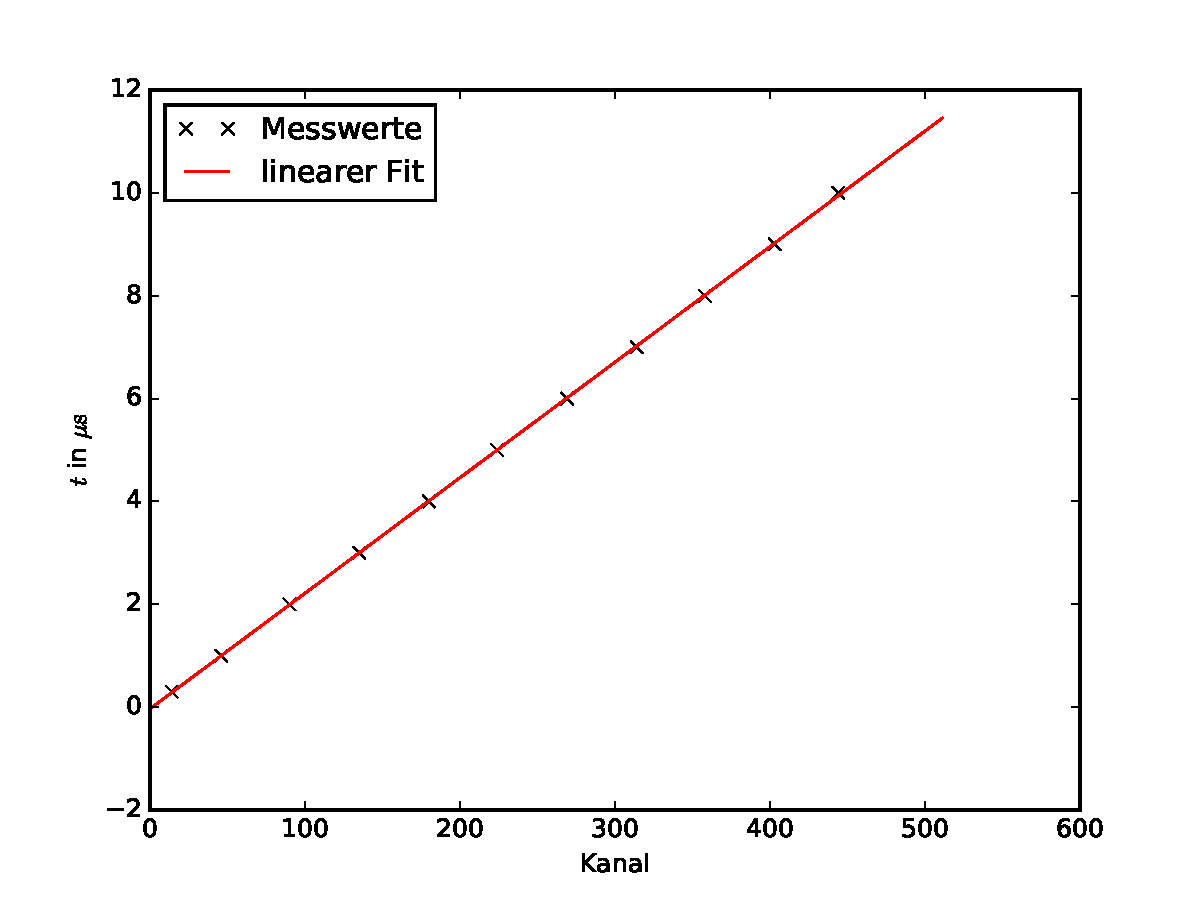
\includegraphics[width = \textwidth]{Pics/Kalibrierung.pdf}
  \caption{Grafische Darstellung der Kanalbelegung und lineare Regression.}
  \label{fig:Kalibrierung}
\end{figure}

\begin{equation}
  T(K) = A*K + B
  \label{eqn:Kalibrierung_Fit}
\end{equation}

Mithilfe von Formel \eqref{eqn:Kalibrierung_Fit} wird eine lineare Regression
durchgeführt, um zu ermitteln, zu welchem Kanal welcher zeitliche Abstand gehört.
Für die Parameter A und B ergeben sich dabei folgende Wert:

\begin{align}
  A &= (0.02247 \pm 0.00005) \,\, \su{\mu s} \\
  B &= (-0.032 \pm 0.014) \,\, \su{\mu s}
\end{align}

\subsection{Bestimmung der Lebensdauer von kosmischen Myonen}

In dem letzten Abschnitt der Auswertung wird die Lebensdauer der Myonen bestimmt.
Die Messung wurde über einen Zeitraum von $T\ua{ges} = 81591$ $\su{s}$ durchgeführt.
Dabei wurden $N\ua{Start} = 1444133$ Startimpulse registriert sowie $N\ua{Stop} =
4255$ Stopimpulse. Die eingestellte Suchzeit beträgt $T\ua{Search} = 10 \, \su{\mu s}$.
Mit diesen Werten lässt der Untergrung berechnen.

\begin{align}
  R &= \frac{N\ua{Start}}{T\ua{ges}} = 17.7 \,\, \frac{\su{Impulse}}{\su{s}}
  \label{eqn:Rate} \\
  N\ua{Search} &= R \cdot T\ua{Search}
  \label{eqn:Nnull}\\
  W(1) &= N\ua{Searcg} \cdot \exp{N\ua{Search}}
  \label{eqn:w1}\\
  U\ua{ges} &= W(1) \cdot N\ua{Start}
  \label{eqn:U1}
\end{align}

Zuerst wird die Rate der pro Sekunde ausgelösten Startsignale bestimmt \eqref{eqn:Rate},
mit der dann die Anzahl von in der Suchzeit ausgelösten Signale \eqref{eqn:Nnull}
bestimmt wird. In der Versuchsanleitung wurde angegeben, dass die Wahrscheinlichkeit,
dass k Myonen in der Suchzeit eintreffen gemäß einer Poisson-Verteilung gegeben ist.
Somit ergibt sich für die Wahrscheinlichkeit, dass ein Myon eintrifft W = 0.00018 $\%$.
Gemäß Formel \eqref{eqn:U1} lässt sich dann die Anzahl der dem Untergrund zuzuordnenden
Signale berechnen. Da sich die Untergrund Signale gleich auf jeden Kanal verteilen,
ergeben sich pro Kanal $U\ua{1} = 0.499$ Signale.

\begin{figure}
  \includegraphics{Pics/Spektrum_groß.pdf}
  \caption{Gemessene Anzahl an Impulsen pro Kanal.}
  \label{fig:Spek_groß}
\end{figure}

Im folgenden wird dieser Wert jedoch nicht verwendet, sondern lediglich mit einem
durch die Regression ermittelten Wert verglichen. Die gemessene Verteilung der
Stopsignale auf die Kanäle ist in Tabelle \ref{tab:Spektrum} dargestellt. Für die
Auswertung wurden
dabei alle Kanäle vernachlässigt, deren gemessener Wert 0 ist. Jedem Kanal mit
der Anzahl $n$ wird als Fehler $\sqrt{n}$ zugeteilt. Da hier ein gewichteter
Fit durchgeführt wird, würden dabei Werte mit Fehler 0 eine Singularität hervorrufen.

\begin{equation}
  N(t) = N\ua{0} \cdot \exp{-\lambda \cdot t} + U\ua{2}
  \label{eqn:Exponentiell}
\end{equation}

Für die Auswertung der in Abbildung \ref{fig:Spek_groß} dargestellten Werte wird an die Funktion
\eqref{eqn:Exponentiell} gefittet. Für die Parameter ergeben sich somit folgende
Werte:

\begin{align}
  N\ua{0} &= (42 \pm 1) \\
  \lambda &= (0.558 \pm 0.018) \cdot 10^{6}\, \frac{1}{\su{s}} \\
  U\ua{2} &= (1.02 \pm 0.13)
\end{align}

Durch die bestimmte Zerfallskonstante $\lambda$ lässt sich dann die mittlere
Lebensdauer $\tau$ der Myonen bestimmen:

\begin{equation}
  \tau = \frac{1}{\lambda} = (1.79 \pm 0.06) \, \su{\mu s}.
\end{equation}

\input{'Messwert_table.tex'}
